\newcommand\version{v2}
\problemname{Städer}
I ett fjärran kungarike finns $N$ städer numrerade från $0$ till $N-1$.
Städerna är anslutna till varandra med $N-1$ gator som går att använda i båda riktningarna.
Alla gator är lika långa och ansluter exakt två städer på ett sådant sätt att det finns en unik väg mellan alla par av städer.

För två städer $A$ och $B$, låt $L(A, B)$ vara antalet gator på den unika vägen mellan städerna $A$ och $B$. 
Givet ett heltal $K$, hur många par av städer $A, B$ finns det så att $L(A, B) ) K$?

\section*{Exempel}
Låt kungariket ha $N = 5$ städer, anslutna av gator som i figuren:
\begin{figure}[h!]
  \centering
  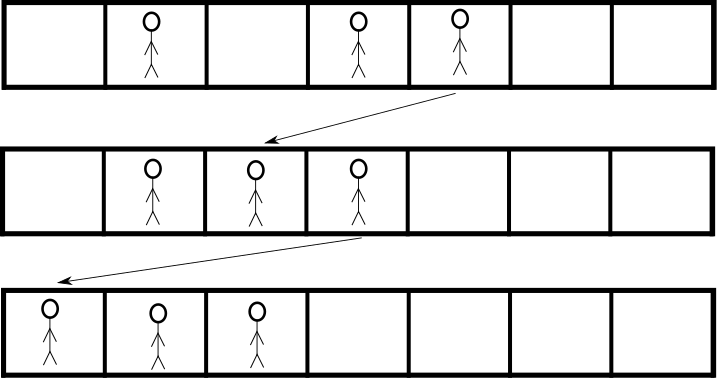
\includegraphics[width=0.3\textwidth]{sample.png}
  \caption{Illustration av exemplet}
\end{figure}

Följande 4 par har en enda gata mellan sig: $(0, 1), (0, 2), (0, 4), (3, 4)$.

Följande 4 par har två gator mellan sig: $(0, 3), (1, 2), (1, 4), (2, 4)$.

Följande 2 par har tre gator mellan sig: $(1, 3), (2, 3)$.

Det innebär att för $K = 1, 2, 3$ skulle svaren vara $4, 4, 2$ respektive.

\section*{Uppgift}
Uppgiften är att beräkna hur många par av städer som har precis $K$ gator mellan sig. Du ska implementera funktionen \texttt{paths(N, K, F, T)}.
\begin{itemize}
  \item \texttt{paths(N, K, F, T)} - den här funktionen kommer att anropas precis en gång av domaren.
  \begin{itemize}
    \item \texttt{N}: antalet städer i kungariket.
    \item \texttt{K}: antalet vägar mellan par av städer som vi är intresserade av.
    \item \texttt{F}: en array med $N-1$ element \texttt{F[i]} ($0 \le i < N$) innehåller den ena staden som den $i$:te gatan är ansluten till.
    \item \texttt{F}: en array med $N-1$ element \texttt{F[i]} ($0 \le i < N$) innehåller den andra staden som den $i$:te gatan är ansluten till.
    \item Det är alltid möjligt att färdas mellan varje par av städer med hjälp av gatorna.
    \item Funktion ska returnera antalet par av städer med precis $K$ gator mellan sig.
  \end{itemize}
\end{itemize}

\section*{Delpoäng}
Problemet består av flera grupper av testfall. Varje grupp ger ett visst antal poäng och för att klara det måste du klara alla testfall i gruppen.

\begin{tabular}{|l|l|l|}
  \hline
  \textbf{Grupp} & \textbf{Poäng} & \textbf{Gränser} \\ \hline
  1 & 9 & $1 \le K \le N \le 100$ \\ \hline
  2 & 19 & $1 \le K \le N \le 1\,000$ \\ \hline
  3 & 34 & $1 \le K \le 10$, $N \le 100\,000$ \\ \hline
  4 & 38 & $1 \le K \le N \le 100\,000$ \\ \hline
\end{tabular}

\section*{Input format}
Exempeldomaren läser indata i följande format:

\begin{itemize}
  \item rad $1$: \texttt{N K}
  \item rad $2$: \texttt{F[0] F[1] .. F[N - 2]}
  \item rad $3$: \texttt{T[0] T[1] .. T[N - 2]}
\end{itemize}

\section*{Output format}
Exemepeldomaren skriver ut en rad med värdet som returnerades av \texttt{paths(N, K, F, T)}.
